\section{架构与实验细节}\label{app:architecture}

因果 Grassmann 分支使用局部的过去--当前词元对，而不使用未来词元对。词元嵌入 $h_t\in\mathbb R^d$ 被降维为 $z_t=W_{\mathrm{red}}h_t+b_{\mathrm{red}}\in\mathbb R^r$。对于 $\mathcal D_t=\{\Delta\in\{1,2,4\}:t-\Delta\geq0\}$，方向为 $z_{t-\Delta}\rightarrow z_t$，外积坐标为
\begin{equation}
p_{ij,t}^{(\Delta)}=z_{t,i}z_{t-\Delta,j}-z_{t,j}z_{t-\Delta,i},\quad i<j.
\end{equation}
共有 $r(r-1)/2$ 个坐标。子空间的背景遵循 Grassmann 流形上的基等价性~\citep{edelman1998geometry}。几何代数参考资料介绍了 Pl\"ucker 坐标的外积解释。\footnote{\url{https://cs.uwaterloo.ca/~smann/GA/plucker_coordinates.html}；仅用于背景介绍，不作为 KD 的证据。}
线性相关向量的外积为零；归一化仍保持有限：
\begin{equation}
\widehat p_t^{(\Delta)}=\frac{p_t^{(\Delta)}}{\max(\|p_t^{(\Delta)}\|_2,\epsilon)},\quad\epsilon=10^{-8}.
\end{equation}
几何投影先于有效窗口均值计算：
\begin{align}
g_t^{(\Delta)}&=W_{\mathrm{plu}}\widehat p_t^{(\Delta)}+b_{\mathrm{plu}},\\
g_t&=\frac{\sum_{\Delta\in\mathcal D_t}g_t^{(\Delta)}}{\max(1,|\mathcal D_t|)}.
\end{align}
空窗口的输出为零。混合使用依赖特征的向量门控：
\begin{align}
a_t&=\sigma(W_{\mathrm{gate}}[h_t;g_t]+b_{\mathrm{gate}}),\\
h_t^{\mathrm{mix}}&=a_t\odot h_t+(1-a_t)\odot g_t.
\end{align}
该核心模块外围包含 LayerNorm、dropout 和残差前馈处理。LM head 独立于 Transformer logits 生成 G logits；标量 $\alpha$ 仅用于后融合（式~\ref{eq:teacher-fusion}）。图~\ref{fig:teacher_architecture} 为通用示意图，不固定 $\alpha=0.5$。

主要实验使用的小型混合学生模型具有六层网络、宽度 224、八个 Transformer 注意力头、降维宽度 56 和 dropout 0.1，并在最后一个模块进行融合。其参数量为 31,434,257。本地 GPT-2 分词器的词表大小为 50,257，不添加特殊词元。主要实验的教师模型配置见附录~\ref{app:protocols}。该架构是既有实验平台，并非几何特定的方法贡献。

\begin{figure*}[!t]
\centering
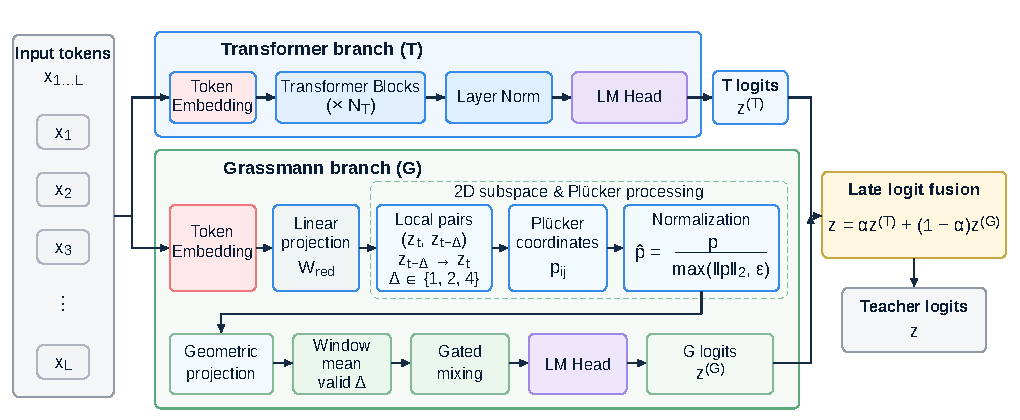
\includegraphics[width=\textwidth]{figures/figA1_teacher_architecture.pdf}
\caption{通用异构教师模型。Grassmann 路径使用因果局部词元对、归一化 Pl\"ucker 坐标、几何投影、有效窗口平均、门控混合及 LM head。后融合在 logits 上进行，$\alpha$ 为自由参数。该架构不能证明几何 KD 的优越性。}
\label{fig:teacher_architecture}
\end{figure*}
